\chapter{System eliminacji zakłóceń}
\section{Wstęp}
\paragraph{}
Realizacja systemu eliminacji zakłóceń w odbiorniku polegała na stworzeniu elementu kompatybilnego z radiem USRP. Modułu, który pobiera sygnał z radia i dokonuje przetwarzania, a wynik tego przekierowuje do demodulatora.
Przetwarzanie zakłada filtrację adaptacyjną w oparciu o algorytm LMS.
\subsection{Środowisko GnuRadio}
Głównym środowiskiem wspierającym radio USRP jest GnuRadio. GnuRadio pozwala na implementacje własnych bloków w oparciu o języki programowania Python i C++. W jego skład wchodzi narzędzie o nazwie \texttt{gnuradio-companion}, które służy do budowy diagramów z bloków o różnym przeznaczeniu. Czynniki te były kluczowe w podjęciu decyzji o doborze tego narzędzia do realizacji projektu.
\paragraph*{Diagramy}
    Diagram nazywany jest również projektem i łączy się z wielu bloków funkcjonalnych.
    Zawiera przynajmniej jedno źródło i jedno ujście sygnału.
    Tworzy łańcuch w którego ogniwach zachodzi przetwarzanie sygnału.
    Nadzoruje poprawność połączeń i zarządza wykonywaniem programu.
\paragraph*{Bloki}
    Mogą być źródłem sygnału (np. generator), ujściem (np. wyjście audio w PC) lub elementem pośredniczącym (np. filtry) w procesie przetwarzania. 
    Każdy z bloków określa swój typ danych wejściowych i wyjściowych, co ogranicza możliwość połączeń, lecz gwarantuje kompatybilność typów.

\section{Blok funkcjonalny}
\subsection{Założenia}
\paragraph{}
Pierwszym założeniem projektowym bloku było zapewnienie interfejsu zgodnego ze schematem filtra. 
Powinien posiadać dwa wejścia: dla sygnału zakłóconego i sygnału odniesienia. 
Wyjścia również dwa: pierwsze- sygnału odfiltrowanego, drugie- wektora błędu do monitorowania szybkości zbieżności algorytmu.

Kolejny parametr określa liczbę próbek wyjściowych do wejściowych.
Blok nie będzie wpływał na liczbę próbek sygnału wejściowego, zatem stosunek $n_{wej}/n_{wyj}$ powinien wynosić $1:1$. 
W nomenklaturze środowiska GnuRadio takie przetwarzanie określa się jako synchroniczne.

Typem danych wejściowych jak i wyjściowych będą wartości zespolone próbek.
Parametrami do ustawienia przez użytkownika w środowisku graficznym będą:
\begin{enumerate}
 \item rząd $N$ filtru w postaci liczby całkowitej 
 \item długość kroku $\mu$ w postaci liczby zmiennoprzecinkowej
 \item liczba iteracji w postaci liczby całkowitej
 \item początkowe współczynniki filtra w postaci wektora liczb o długości N 
 \end{enumerate}
 
Parametry zostaną podzielone na wymagane (1, 2) i opcjonalne (3, 4)
\subsection{Szablon projektu}
\paragraph{}
Środowisko GnuRadio dostarcza szereg narzędzi wspomagających pracę w rozwijaniu własnych modułów tak, aby były kompatybilne z już istniejącymi. 
Jednym z nich jest \texttt{gr\_modtool}, który został wykorzystany do stworzenia struktury plików bloku filtra adaptacyjnego. 
Dzięki temu nasz blok będzie w stanie łączyć się z innymi, przekazywać i odbierać sygnały oraz będzie rozumiał polecenia wydawane przez środowisko w którym zostanie umieszczony. 
W projekt włącza się katalog z testami jednostkowymi, sprawdzającymi elementarne funkcjonalności bloku. 
Dobrze zaimplementowane i przemyślane testy jednostkowe informują o wykrytych błędach powstających podczas tworzenia algorytmu.
Oprócz testów w projekcie tworzy się plik \texttt{.xml}, który określa reprezentację bloku w środowisku graficznym \texttt{gnuradio-companion}. 
W zależności od wybranego języka programowania, również plik z kodem źródłowym bloku.
\subsection{Klasa obiektu bloku}
\paragraph{}
Serce modułu odpowiedzialnego za przetwarzanie wejściowych strumieni danych znajduje się w pliku  \texttt{adaptive\_lms\_filter\_cc.py}. W tym miejscu zdefiniowana jest klasa bloku wraz z jej zmiennymi i funkcjami.

\paragraph{}
\begin{tabular}{|l|} \hline
\texttt{adaptive\_lms\_filter\_cc} \\
\hline
\texttt{-input\_items} \\
\texttt{-output\_items} \\
\texttt{-weights} \\
\texttt{-order} \\
\texttt{-step} \\
\texttt{-num\_of\_iter} \\
\hline
\texttt{+work()} \\
\texttt{+consume()} \\
\texttt{+set\_history()} \\
\hline
\end{tabular}

\paragraph{}
Funkcja \texttt{work} uruchamiana cykliczne przez proces \texttt{scheduler} zawiera instrukcje odpowiedzialne za całe przetwarzanie wewnątrz bloku. 
Jest miejscem w którym należy umieścić implementację filtra. 
Pobiera z wejścia nadchodzące elementy i na ich postawie oblicza produkty, które kieruje na wyjście.

Należy zauważyć, że w niektórych przypadkach do obliczenia wartości próbki wyjściowej potrzeba więcej niż jedną próbkę wejściową. 
Jest tak w przypadku filtracji, gdzie filtr o długości $N$ potrzebuje $N-1$ próbek minionych. 
Konieczne jest stworzenie bufora z którego można będzie pobierać te wartości. 
Funkcja \texttt{set\_history} tworzy miejsce do przechowywania wcześniejszych próbek w pamięci, a jako parametr przyjmuje długość tego bufora.

\subsection{Inicjalizacja}
\paragraph{}
Następuje zawsze po uruchomieniu projektu. 
W każdym bloku (obiekcie) na diagramie tworzą się instancje do których przypisuje się wartości początkowe.
Parametry mogą być dostosowywane przez użytkownika na etapie projektowania (w czasie przed uruchomieniem), lub zmieniane w trakcie wykonywania programu.
Zmiana parametrów w biegu wiąże się z ponowną inicjalizacją bloku i może prowadzić do utraty danych przechowywanych wewnątrz tego obiektu. 
W środowisku \texttt{gnuradio-companion} okno właściwości pojawia się po podwójnym kliknięciu na blok. 
Zamiast stałej wartości parametru można przypisać referencję do jednego z dostępnych elementów sterujących np. suwaka lub pokrętła. 
Dzięki temu dostosowywanie bloku możliwe jest z poziomu graficznego panelu użytkownika (R).

\begin{figure}[t]
\centering
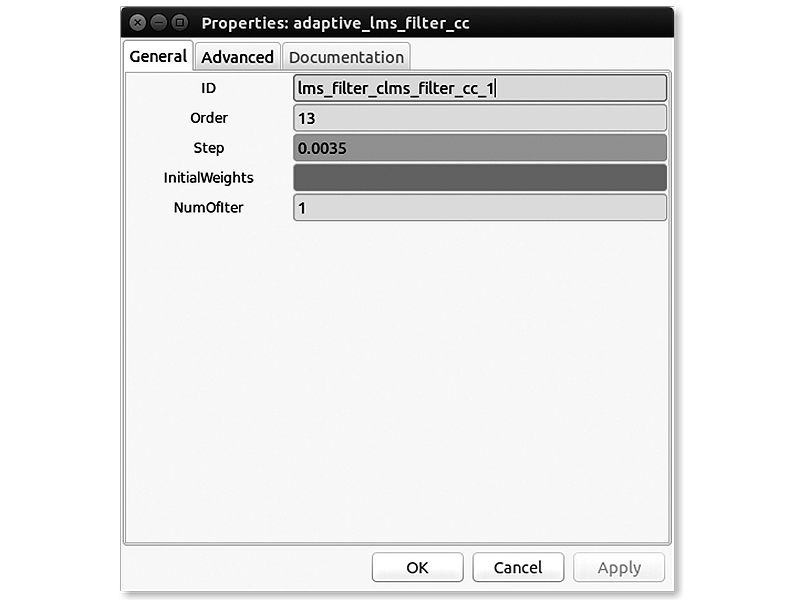
\includegraphics[scale=1]{properties.png}
\caption{Panel parametrów bloku}
\label{blockproperties}
\end{figure}

Projekt pozwala na sterowanie dwoma parametrami podczas pracy filtra:
\begin{enumerate}
\item \texttt{order} - rząd $M = \{5,6,...,30\}$
\item \texttt{step} - krok adaptacji $\mu \in [0.0002, 0.005]$
\end{enumerate}

\subsection{Implementacja}
\paragraph{}
Nieodłączną częścią modułu wykorzystywaną przez \texttt{gnuradio-companion} jest plik \texttt{adaptive\_lms\_filter\_cc.xml}, który określa parametry wejściowe bloku, układ doprowadzeń i wyprowadzeń; gwarantuje kompatybilność połączeń z innymi blokami przez definiowanie typów danych dla wszystkich wejść, wyjść i parametrów. 
Pozwala również ustawić właściwości istotne dla poprawnego kategoryzowania w zasobach bibliotek.

Poniżej fragment struktury pliku \texttt{.xml}:


\begin{verbatim}

<?xml version="1.0"?>
<block>
  <name>adaptive_lms_filter_cc</name>
  <key>lms_filter_adaptive_lms_filter_cc</key>
  <category>[lms_filter]</category>
  <import>import lms_filter</import>
  <make>lms_filter.adaptive_lms_filter_cc
  ($order, $step, $weights $num_of_iter)</make>

  <param>
    <name>Order</name>
    <key>order</key>
    <type>int</type>
  </param>

  <param>
    <name>Step</name>
    <key>step</key>
    <type>float</type>
  </param>

  <sink>
    <name>reference</name>
    <type>complex</type>
  </sink>

  <source>
    <name>out</name>
    <type>complex</type>
  </source>
\end{verbatim}

Nazwy parametrów zostały dobrane tak, aby blok dobrze integrował się ze środowiskiem i mógł zostać powtórnie wykorzystany w projektach innych użytkowników. Stąd język angielski, jako wspólny dla inżynierów na całym świecie. 

\paragraph{Algorytm}

Aby zwiększyć efektywność i wygodę działań algebraicznych na macierzach, zastosowano narzędzia \texttt{numpy} będące rozszerzeniem języka Python.

Algorytm pobiera z dwóch wejść próbki sygnałów i zapisuje je do bufora o wymiarze $b = 2 \times M$, którego każdy wiersz to jeden sygnał, a każda kolumna to kolejna próbka tego sygnału. 
Filtr odczytuje z bufora, wykonuje operacje algebraiczne, adaptacyjnie zmieniając swoje współczynniki. 
Odfiltrowany sygnał przekierowywany jest na wyście, a z bufora wymazywane są próbki $b_{1M}, b_{2M}$.
\begin{samepage}
\begin{algorithmic}
\Require $w \gets w_0 \gets [0, 0,...,0]^{T}$,
\State buffer $\gets $ \Call{Set History}{$2 \times M$}
\While {Program running}
    \Repeat\ buffer $\gets$ \Call{Consume samples}{reference input, noisy signal input} \Until buffer length $<$ filter order
    \State \Call {Filter}{buffer}
    \State \Call {Remove From Buffer}{oldest $x, d$}
\EndWhile
\Function{Filter}{samples}
\ForAll {$x, d \gets$ samples}
    \State $y \gets x \cdot w$
    \State $e \gets d - y$
    \State $w \gets  w \cdot step \cdot x \cdot e$
    \State $y \gets x \cdot w$
    \State \Return $y, e$
\EndFor
\EndFunction
\Function{Consume samples}{reference input, noisy signal input}
    \State $x \gets$ reference input
    \State $d \gets$ noisy signal input
    \State buffer $\gets x, d$
    \State \Return buffer
\EndFunction
\end{algorithmic}
\end{samepage}


\subsection{Instalacja}

Kiedy wszystkie wymagane funkcjonalności zapisane w kodzie pomyślnie przechodzą etap testowania, implementację uznaje się za zakończoną.
Moduł należy dołączyć do bibliotek GnuRadio, aby jego graficzna reprezentacja znalazła się w środowisku \texttt{gnuradio-companion}, a sam blok mógł zostać wykorzystany jako element w systemie odbiornika.

Proces instalacji nadzoruje narzędzie \texttt{cmake}, które wykonuje instrukcje z pliku \texttt{Makefile} powstałego podczas tworzenia szablonu projektu. Gotowy blok przedstawia Rysunek \ref{grcblock}. 

\begin{figure}[ht]
\centering
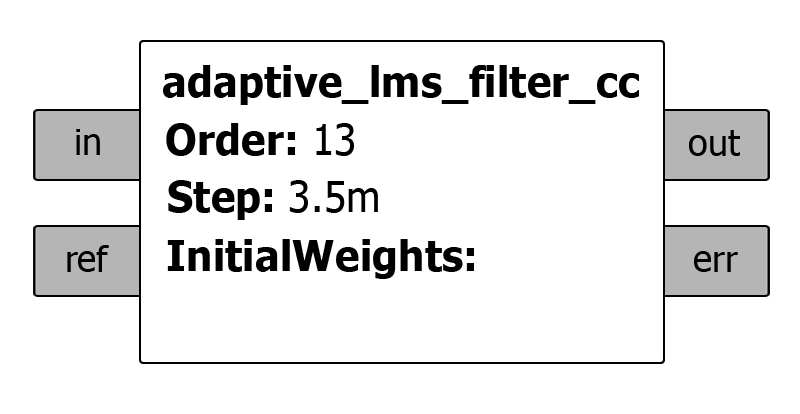
\includegraphics[scale=0.3]{block.png}
\caption{Reprezentacja graficzna bloku w \texttt{gnuradio-companion}}
\label{grcblock}
\end{figure}
